\chapter[Energia]{Energia}

O sistema de energia será responsável por realizar a alimentação dos módulos propostos no projeto, além de dimensionar os cabeamentos de lógica que interconectarão os componentes eletrônicos.

As estações de medição serão alimentadas por um sistema fotovoltaico off-grid com o intuito de torná-las autônomas e permitir que elas possam ser instaladas longe da fonte de alimentação principal da fazenda. Assim, será apresentado o sistema fotovoltaico demonstrando seu funcionamento e todos os equipamentos que o compõem desde a geração da energia até a distribuição para o resto da estação.

Além disso, será apresentado a proposta de alimentação para o módulo atuador que será responsável por acionar ou desligar a irrigação automaticamente e para a central de comando.  

\section{Sistemas Fotovoltaicos Autônomos}

	Os Sistemas Fotovoltaicos Autônomos ou Isolados são sistemas de geração de energia elétrica a partir de ondas de radiação eletromagnética solar que atingem a superfície terrestre, aplicados em locais que não possuem uma conexão com a rede elétrica de distribuição. Os principais componentes existentes neste tipo de sistema são um conjunto de placas fotovoltaicas, um controlador de carga, um banco de baterias, e a depender da aplicação, um inversor CC-CA de tensão contínua para tensão alternada. 

\begin{figure}[H]
		\centering
		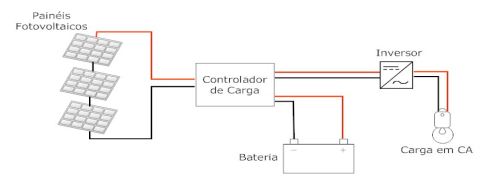
\includegraphics[width = .5 \textwidth]{energia/figuras/ene_pc1_01}
		\caption{Representação de um sistema fotovoltaico autônomo. Fonte:\cite{Antonio}}
		\label{ene_pc1_01}
	\end{figure}	 		

	Os painéis fotovoltaicos possuem a função de converter a luz solar em eletricidade, na forma de tensão e corrente contínua. Já o controlador de carga tem a função de regular a carga da bateria e prolongar a sua vida útil, além de proteger o banco de descargas e sobrecargas excessivas. Os bancos de baterias são usados para o armazenamento da energia gerada para uso posterior em períodos de pouca ou nenhuma geração. Os inversores são usados em sistemas autônomos cuja a carga exija tensão e corrente alternada CA.
		
	Os fenômenos que afetam a radiação solar no seu percurso através da atmosfera são o principal problema para se quantificar a disponibilidade energética. Quando esta energia entra na atmosfera, existem dois tipos de fenômenos que vão influenciar o seu percurso: a geometria do Sol/Terra e os fatores meteorológicos. Estes serão os responsáveis por uma atenuação na quantidade de energia que poderia chegar até a superfície terrestre. \cite{Sofia}
	
	O estudo da geometria do Sol/Terra visa conhecer a posição do Sol no céu e a partir dela determinar como os raios solares incidem sobre a superfície do módulo fotovoltaico. Devido a posição do Sol variar ao longo do dia e do ano, existem certas variáveis necessárias para determinar a posição dos paineis, como por exemplo, os ângulos azimutal, zenital e o ângulo de altura solar. \cite{Villalva}
	
\begin{figure}[H]
		\centering
		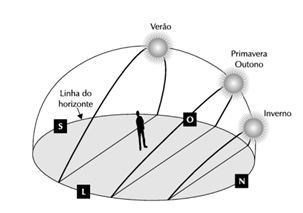
\includegraphics[width = .5 \textwidth]{energia/figuras/ene_pc1_02}
		\caption{A trajetória do movimento aparente do Sol é diferente ao longo do ano. Fonte: \cite{Villalva}}
		\label{ene_pc1_02}
	\end{figure}	
	
\begin{figure}[H]
		\centering
		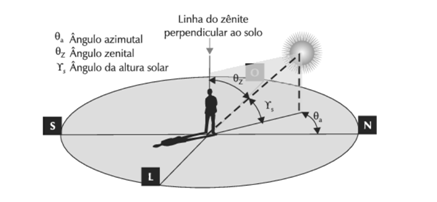
\includegraphics[width = .5 \textwidth]{energia/figuras/ene_pc1_03}
		\caption{A posição do Sol é definida pelos ângulos azimutal, zenital e da altura solar: Fonte: \cite{Villalva}}
		\label{ene_pc1_03}
	\end{figure}	

Os fatores meteorológicos estão relacionados às perdas que a radiação solar sofre ao percorrer a atmosfera terrestre devido aos fenômenos de absorção, reflexão e dispersão. Por causa disto as características da radiação solar que chega ao solo dependem da espessura da camada de ar e da composição da atmosfera, incluindo o ar e os elementos suspensos. A radiação que acaba atingindo a superfície terrestre, denominada aqui por radiação global, é a soma da radiação direta que vêm do Sol e da radiação difusa que alcança o plano terrestre de forma indireta por conta dos componentes do ar ou de outras matérias e estruturas próximas do plano de referência terrestre. \cite{Villalva}

	Grande parte dos sistemas fotovoltaicos existentes apresentam ângulos de inclinação do módulo fixo. Idealmente, o melhor aproveitamento da energia solar ocorre quando o ângulo de incidência dos raios solares, mostrado na figura \ref{ene_pc1_04}, é igual a zero. Para um módulo com um ângulo de inclinação fixo isso não é possível de obter. Portanto para esses casos a melhor forma de instalar um módulo fotovoltaico fixo é orientá-lo com sua face para o norte geográfico, e determinar o seu ângulo de inclinação de acorda com a latitude geográfica do sistema fotovoltaico. Este critério de instalação e inclinação do módulo fotovoltaico é recomendado por muitos fabricantes de placas. A tabela \ref{ene_pc1_01_tab} mostra a escolha do ângulo de inclinação recomendado para o módulo fotovoltaico com base em sua latitude geográfica.
	
	
\begin{figure}[H]
		\centering
		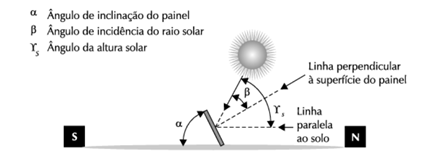
\includegraphics[width = .5 \textwidth]{energia/figuras/ene_pc1_04}
		\caption{ Ângulo de inclinação e incidência dos raios solares.Fonte: \cite{Villalva}}
		\label{ene_pc1_04}
	\end{figure}	
	
\begin{table}
\centering
\caption{Angulação dos painéis}
\begin{tabular}{|c|c|}
\hline 
Latitude georgáfica do local & ângulo de inclunação recomendado \\ 
\hline 
$0\,^{\circ}\mathrm{C}$ a $10\,^{\circ}\mathrm{C}$& $10\,^{\circ}\mathrm{C}$ \\ 
\hline 
$11\,^{\circ}\mathrm{C}$ a $20\,^{\circ}\mathrm{C}$&  latitude\\ 
\hline 
$21\,^{\circ}\mathrm{C}$ a $30\,^{\circ}\mathrm{C}$& latitude + $5\,^{\circ}\mathrm{C}$\\ 
\hline 
$31\,^{\circ}\mathrm{C}$ a $40\,^{\circ}\mathrm{C}$ &  latitude + $10\,^{\circ}\mathrm{C}$\\ 
\hline 
mais de $40\,^{\circ}\mathrm{C}$ &  latitude + $15\,^{\circ}\mathrm{C}$ \\ 
\hline 
\end{tabular} 
\label{ene_pc1_01_tab}
\end{table}	
	
\subsection{Módulo Fotovoltaico} 

	Atualmente existem várias tecnologias para a fabricação de células e módulos fotovoltaicos, sendo as mais comuns e que dominam o mercado as tecnologias de células fotovoltaicas de silício monocristalino, de silício policristalino e as de filme fino de silício. 
	
	Um módulo fotovoltaico é uma estrutura composta por um conjunto de células fotovoltaicas conectadas eletricamente entre si, onde a quantidade de células determina a potência do módulo. Geralmente os módulos fotovoltaicos de silício cristalino são encontrados no mercado numa faixa de potência de 10 W a 330 W.
	
	A transformação da energia solar em energia elétrica ocorre graças ao fenômeno físico denominado de efeito fotovoltaico. Esse fenômeno acontece quando a radiação eletromagnética do Sol incide em uma célula composta de materiais semicondutores com propriedades específicas. Esse processo requer em primeiro lugar, um material em que a absorção da luz gera pares de elétrons – lacunas. Então, para que esse processo aconteça uma célula fotovoltaica é composta tipicamente pela junção de duas camadas de material semicondutor, uma do tipo P (com falta de elétrons) e outra do tipo N (com excesso de elétrons). Quando essa junção semicondutora é feita ocorre uma mudança dos elétrons e lacunas de uma camada para outra, que origina um campo elétrico e cria uma barreira potencial entre as duas camadas. \cite{Bluesol}
	
	Com essa estrutura sendo exposta a luz solar, os elétrons que migraram para a camada P adquirem energia suficiente para superarem a barreira potencial e movimentar-se, onde esses elétrons em movimentos são coletados pelos eletrodos metálicos localizados na frente da célula, e existindo um circuito fechado, os elétrons vão circular em direção aos eletrodos da camada N formando uma corrente elétrica. \cite{Villalva}

	
\begin{figure}[H]
		\centering
		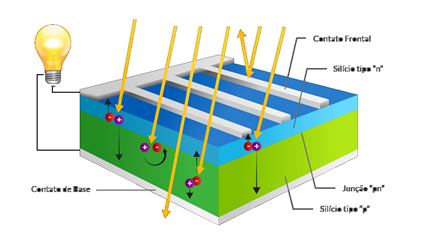
\includegraphics[width = .5 \textwidth]{energia/figuras/ene_pc1_05}
		\caption{Esquemático de uma célula solar padrão de junção P-N. Fonte: \cite{Bluesol}}
		\label{ene_pc1_05}
	\end{figure}	


	Uma célula fotovoltaica pode ser representada por um circuito elétrico equivalente ilustrado a seguir.
	
	
\begin{figure}[H]
		\centering
		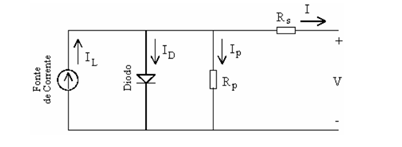
\includegraphics[width = .5 \textwidth]{energia/figuras/ene_pc1_06}
		\caption{Circuito equivalente incluindo as resistências parasitas de uma célula solar. Fonte: \cite{Hecktheuer}}
		\label{ene_pc1_06}
	\end{figure}

		Os efeitos resistivos em células solares reais reduzem a eficiência, dissipando potência nas resistências. As resistências parasitas mais comuns estão representadas no circuito anterior, e são a resistência em cadeia Rs e a resistência de derivação Rp. A resistência em cadeia é referente ao movimento de elétrons nos semicondutores da célula e nos eletrodos metálicos, já a resistência de derivação é em relação a caminhos de corrente alternativo para a corrente gerada pela luz nas células fotovoltaicas. \cite{Campesato}
	
	A junção P-N funciona como um diodo, e a corrente interna unidirecional que passa nele depende da tensão V dos terminais da célula. Então, a relação corrente-tensão de um diodo de junção P-N, no escuro e desconsiderando as resistências parasitas, é dada por:
	
	\begin{equation}
	I_{dark} = I_0 . exp(\dfrac{qV}{nkT} - 1)
	\end{equation}
	
	Agora enquanto estiver sob incidência de luz, a característica ideal de corrente-tensão, novamente desconsiderando as resistências parasitas, é:
	
	\begin{equation}
	I = (I_1 - I_0) . exp(\dfrac{qV}{nkT} - 1)
	\end{equation}
	
	Onde, $I_1$ é a corrente gerada na luz, $I_0$ é a corrente de saturação no escuro do diodo, n é o fator de idealidade (tipicamente na faixa de 1 a 2), q é a carga eletrônica do elétron e T é a temperatura em graus Kelvin.
	
	Considerando as resistências parasitas, a equação corrente-tensão é dada por:
	
	\begin{equation}
	I = (I_1 - I_0) . (exp(\dfrac{q(V + RsI)}{nkt} - 1)) - \dfrac{V + RsI}{R_p}
	\end{equation}
	 
	A figura \ref{ene_pc1_07} mostra a curva característica I – V de corrente e tensão em azul, e a  curva característica P - V em vermelho de um módulo fotovoltaico, onde é possível observar o seu ponto de máxima potência, que é o ponto onde a produção de energia do módulo é a maior e têm-se o melhor aproveitamento da energia solar.
	
		
\begin{figure}[H]
		\centering
		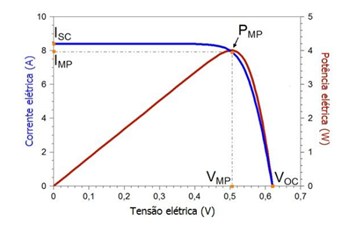
\includegraphics[width = .5 \textwidth]{energia/figuras/ene_pc1_07}
		\caption{Curva característica I-V e P-V de uma célula fotovoltaico de silício cristalino. Fonte:\cite{Cresesb}}
		\label{ene_pc1_07}
	\end{figure}

	A produção de corrente elétrica de um módulo fotovoltaico sofre influência direta da intensidade da radiação solar que incide em suas células solares. Portanto, a corrente máxima que um módulo pode fornecer varia proporcionalmente com a irradiância, logo isso resulta que para pouca luz a corrente produzida pelo módulo é pequena e consequentemente a sua capacidade de gerar energia é reduzida na mesma proporção e de forma significativa. A figura \ref{ene_pc1_08} ilustra a influência da radiação solar.
	
\begin{figure}[H]
		\centering
		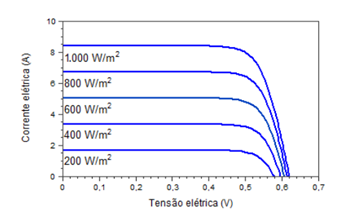
\includegraphics[width = .5 \textwidth]{energia/figuras/ene_pc1_08}
		\caption{Influência da variação da irradiância solar na curva característica I-V de uma célula fotovoltaica de c-Si. Fonte: \cite{Cresesb}}
		\label{ene_pc1_08}
	\end{figure}

	A temperatura de funcionamento do módulo fotovoltaico também influencia o seu desempenho, pois pode alterar a tensão fornecida em seus terminais. Por exemplo, para temperaturas mais baixas as tensões são maiores e em temperaturas mais altas as tensões são menores. Isso é ilustrado na figura \ref{ene_pc1_09} a seguir.
	
		
\begin{figure}[H]
		\centering
		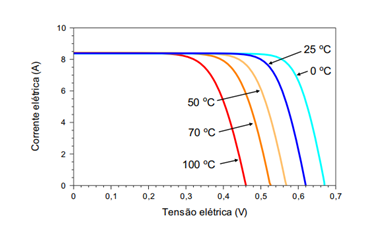
\includegraphics[width = .5 \textwidth]{energia/figuras/ene_pc1_09}
		\caption{ Influência da temperatura da célula fotovoltaica na sua curva característica I-V (para irradiância de 1000 $W/m^2$). Fonte: \cite{Cresesb}}
		\label{ene_pc1_09}
	\end{figure}

\subsubsection{Calculo da energia produzida pelos módulos fotovoltaicos} 

	Para o dimensionamento de um sistema fotovoltaico é extremamente importante determinar o valor de energia produzida diariamente por um módulo fotovoltaico. Existem dois métodos para o cálculo da energia produzida pelo módulo, que são o método da insolação e o método da corrente máxima do módulo. \cite{Villalva}.
	
	\textbf{Método da insolação}
	
	Esse método é empregado no cálculo da energia produzida pelo módulo quando se tem informação sobre a energia do Sol disponível diariamente no local da instalação, ou a insolação do local dada em $Wh/m^2 por dia$. Esse dado da insolação diária pode ser encontrado em mapas solarimétricos ou em uma ferramenta computacional.  
	
	O método da insolação para o cálculo da energia produzida pelo módulo é válido quando se considera o uso de controladores de carga com o recurso do MPPT (rastreamento do ponto de máxima potência). Ao considerar o valor da energia do Sol disponível diariamente como base para o cálculo, espera-se extrair o máximo possível dessa energia, e nesse caso a energia é limitada apenas pela eficiência do módulo. \cite{Villalva}
	
	Logo, a energia produzida pelo módulo fotovoltaico é determinada pela seguinte equação:
	
	\begin{equation}
	E_p = E_s . A_m . n_m
	\end{equation}
	
	Em que, $E_p$ é a energia produzida pelo módulo diariamente (Wh), $E_s$ é a insolação diária ($Wh/m^2 por dia$), $A_m$ a área da superfície do módulo e $n_m$ é a eficiência do módulo.
	
	\textbf{Método da corrente máxima do módulo}
	
	Nesse método considera-se que não é possível ter o aproveitamento máximo da energia solar, pois o sistema fotovoltaico não está equipado com o recurso de MPPT. O sistema é impossibilitado de converter toda a energia produzida ficando condicionada ao ponto de operação imposto pela tensão da bateria ou do banco de baterias do sistema.\cite{Villalva}
	
	A primeira ação para o cálculo da energia produzida pelo módulo por esse método é obter as características do módulo em sua folha de dados. Podem ser usadas as características STC (condições padrão de teste do módulo) ou NOCT (condições normais de temperatura da célula), mas as condições NOCT são as mais recomendadas para uso pois representam com mais proximidade as características reais de operação.
	
	Portanto, o cálculo da energia produzida pelo módulo nesse método é realizada pela seguinte equação:
	
	\begin{equation}
	E_p = P_m . H_s
	\end{equation}
	
	Onde, $E_p$ é a energia produzida pelo módulo diariamente (Wh), $P_m$ é a potência do módulo (W) e $H_s$ são as horas diárias de insolação (horas), no qual Hs é um valor que pode variar ao longo do ano e é diferente para cada região geográfica, mas para esse método Hs está numa faixa de valores de quatro a seis horas.
	
	A potência do módulo é determinada por:
	
	\begin{equation}
	P_m = I_{sc} . V_{bat}
	\end{equation}
	
	Em que, $I_{sc}$ é a corrente de curto-circuito do módulo (A) e geralmente considerada na condição NOCT, e $V_{bat}$ é a tensão da bateria ou do banco de baterias (V).
	
	Para determinar o número total de módulos necessários no sistema, é preciso conhecer a energia diária consumida no sistema ($E_c$) e a energia diária produzida pelo módulo ($E_p$), calculado por:
	
	\begin{equation}
	N = \dfrac{E_c}{E_p}
	\end{equation}
		
	Conhecendo o número de módulos necessários, a ligação e a associação dos módulos dependem da definição da tensão de operação do sistema.
	
	Como para o projeto vamos empregar um controlador de carga com PWM, o método que será utilizado para o cálculo da energia produzida pelo módulo será o da corrente máxima, de forma semelhante ao descrito, para o dimensionamento do sistema.
	 
\subsection{Baterias} 

	As baterias presentes em sistemas fotovoltaicos visam proporcionar fornecimento constante de energia para o consumidor e evitar desperdício da energia gerada quando o consumo é baixo, permitindo seu armazenamento para uso posterior. Na maioria dos sistemas fotovoltaicos isolados a presença de uma bateria também é necessária para estabilizar a tensão fornecida aos equipamentos ou ao inversor, pois a tensão de saída do módulo fotovoltaico não é constante e está sujeita a variações. \cite{Villalva}
	
 Existem vários tipos de baterias elétricas, sendo as mais conhecidas e empregadas em sistemas fotovoltaicos as baterias de chumbo ácido por serem mais economicamente viáveis, mas há outras tecnologias com certas características vantajosas, como as baterias de Níquel-Cádmio (NiCd), Níquel-hidreto metálico (NiMH), íon de Lítio e dentre outras. Para aplicações fotovoltaicas é exigido o uso de baterias estacionárias, pois elas podem suportar centenas de ciclos de descarga e recarga, e foram desenvolvidas para sistemas que precisam de armazenamento de energia para a alimentação de equipamentos elétricos e eletrônicos. As baterias encontradas no mercado possuem níveis de tensão de 12 V, 24 V e 48 V.
	
	A vida útil de uma bateria é caracterizada pelo número de ciclos de carga e descarga que ela pode realizar, e depende fortemente da temperatura de operação e da profundidade de descarga da bateria. As figuras \ref{ene_pc1_10} e \ref{ene_pc1_11} ilustram essa influência.
	
		
\begin{figure}[H]
		\centering
		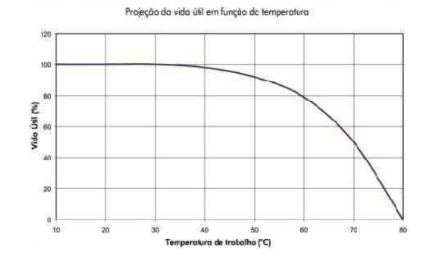
\includegraphics[width = .5 \textwidth]{energia/figuras/ene_pc1_10}
		\caption{Vida útil de uma bateria em função da temperatura de trabalho.Fonte: \cite{Freedom}}
		\label{ene_pc1_10}
	\end{figure}
	
\begin{figure}[H]
		\centering
		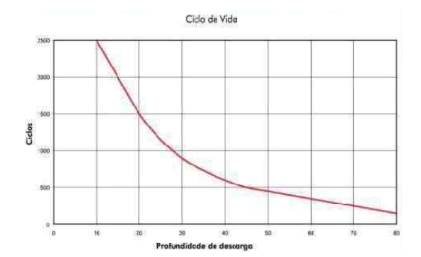
\includegraphics[width = .5 \textwidth]{energia/figuras/ene_pc1_11}
		\caption{Número de ciclos de carga e descarga em função da profundidade de descarga. Fonte: \cite{Freedom}}
		\label{ene_pc1_11}
	\end{figure}


	Das figuras anteriores podemos observar que conforme a temperatura de operação aumenta o tempo de vida da bateria é reduzido de forma considerável, logo sempre é importante verificar as especificações dos fornecedores, que fornecem essas curvas , e tentar projetar a bateria para operar próximo da temperatura indicada pelos fabricantes, que geralmente é na faixa dos 20 a $30\,^{\circ}\mathrm{C}$. Já em relação a profundidade de descarga, observa-se que para profundidades maiores o tempo de vida da bateria é reduzido, agora para uma bateria que se descarregar pouco, ela pode prolongar sua vida útil e seus números de ciclos. A profundidade de descarga é um fator importante no dimensionamento do banco de baterias, e para sistemas fotovoltaicos são recomendadas profundidades na faixa de valores de 20 a 50\%.
	
\subsubsection{Dimensionamento do banco de baterias} 

	Sendo conhecido a energia consumida pela carga diariamente, é possível determinar pelas relações seguintes:

\begin{equation}
	CB_{c20} = \dfrac{E_c . N}{P_d}
\end{equation}

\begin{equation}
	CBI_{c20} = \dfrac{CB_{c20}}{V_{banco}}
\end{equation}

	Onde $CB_{c20}$ é a capacidade de carga do banco de baterias em Wh para o regime de descarga de 20 horas (C20) e $CBI_{c20}$ é a respectiva capacidade de carga do banco em Ah; N é o número de dias de autonomia desejado para o banco de baterias e $V_{banco}$ a tensão do banco de baterias.
	
	O número de baterias em série depende da tensão desejada para o sistema e é determinado pela fórmula:
	
	\begin{equation}
	N_{bs} = \dfrac{V_{banco}}{V_{bat}}
	\end{equation}

	Onde $N_{bs}$ é o número de baterias ligadas em série, $V_{banco}$ a tensão do banco de baterias e $V_{bat}$ a tensão da bateria utilizada.
	
	O número de baterias em paralelo é calculado de modo semelhante pela equação a seguir.
	
	\begin{equation}
	N_{bp} = \dfrac{CBI}{CBI_{bat}}
	\end{equation}
	
	Onde, $CBI_{bat}$ representa a capacidade da bateria selecionada no mesme regime de descarga do valor calculado para CBI.

\subsection{Quadro de proteção e distribuição} 

	No quadro de proteção de corrente contínua do sistema fotovoltaico é onde fica localizado os dispositivos de proteção do sistema. No mesmo quadro de proteção deve estar presente um barramento de aterramento, com a função de coletar as ligações à terra das estruturas metálicas e carcaças dos módulos fotovoltaicos.

	A chave de desconexão ou disjuntor deve estar presente na instalação, devido aos momentos de manutenção do sistema fotovoltaico, permitindo a desconexão dos módulos para garantir a segurança. Tais dispositivos devem suportar níveis de tensão presentes nos sistemas fotovoltaicos e ter a capacidade de interrupção de arco elétrico em corrente contínua. 
	
	O dispositivo de proteção de surto DPS é outro componente importante nos sistemas fotovoltaicos, pois têm a função de proteger os equipamentos e cabos contra sobretensões ocasionadas por descargas elétricas.
	
	
\subsection{Dimensionamento dos cabos de corrente contínua} 

	O cabeamento elétrico empregado nas conexões em corrente contínua devem ser específicos para aplicações fotovoltaicas, e caso opte-se por cabos com isolação convencional, esses devem ser usados em instalações abrigadas em calhas ou eletrodutos. Os cabos para instalações fotovoltaicas possuem proteção a radiação UV e são construídos para suportar temperaturas extremas.
	
	A NBR 5410 indica a bitola adequada para os condutores em função do comprimento do ramal, da tensão nominal e do nível de perdas pretendido. Uma forma alternativa para determinar a seção mínima de um condutor necessária para uma instalação em corrente contínua, é utilizar a seguinte equação \cite{Cresesb}.

\begin{equation}
S  = \rho . \dfrac{d . I}{\delta V} 
\end{equation}

Onde o $\rho$ é a resistividade do material condutor; d a distância total do condutor, considerando o trecho de retorno; I é a corrente que passa pelo condutor e $\delta V$ a queda de tensão tolerada no cabeamento, onde para conexões em cc deve estar entre 1\% e 3\%. É recomendado que a capacidade de condução de corrente do cabo seja 25\% superior à corrente de curto-circuito dos módulos fotovoltaicos em STC.
	
\subsection{Controlador de carga} 

	Segundo CRESESB em seu Manual de Engenharia para Sistemas Fotovoltaicos de 2014 o controlador de carga é um elemento essencial para todo sistema fotovoltaico que utilize armazenamento de energia em sistemas de baterias. Este componente permite otimizar o funcionamento das baterias, proteger suas células de carga e aumentar sua vida útil. 
	
	Desta forma, o controlador de carga é responsável por desconectar a alimentação proveniente do gerador fotovoltaico quando as baterias estiverem em carga plena, além de interromper o fornecimento de energia a carga quando as baterias atingirem um nível mínimo de segurança. Dependendo do controlador, ele pode apresentar mais funções como monitoramento do desempenho do SFI (parâmetro de desempenho de carregamento da bateria), acionar alarmes em caso de problemas e ainda monitorar a temperatura com o objetivo de compensar seu efeito nos parâmetros da bateria. \cite{Cresesb}. 
	
Para especificar o modelo de controlador de carga que melhor atende a uma aplicação é necessário saber o tipo de bateria que será utilizada e o regime de operação do sistema a ser alimentado. Há diversas tecnologias de controladores no mercado de forma que foi pesquisado os principais modelos e analisadas suas características para utilização no projeto. 

	\textbf{Controlador de carga em série}

	O controlador de carga em série pode ser representado pelo esquemático apresentado na figura a seguir:

	\begin{figure}[H]
		\centering
		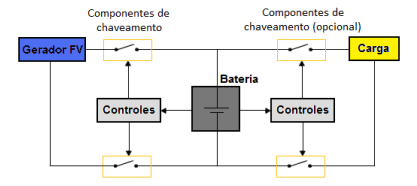
\includegraphics[width = .5 \textwidth]{energia/figuras/ene_pc1_13}
		\caption{Controlador de carga em série. \cite{Cresesb}}
		\label{ene_pc1_13}
	\end{figure}
	

	Este componente pode utilizar um relé eletromecânico ou um dispositivo semicondutor para realizar o chaveamento de proteção da bateria. Nos momentos em que o consumo da carga é baixo e a geração fotovoltaica é alta, os painéis são desconectados e não transmitem a energia produzida para as baterias implicando em perda de eficiência para o sistema como um todo. \cite{Cresesb}.
	
	Vale ressaltar que nem todos os controladores comerciais deste tipo possuem o par de chaves para desconectar a carga da bateria quando o nível mínimo de segurança é atingido. 
	
	\textbf{Controlador de carga em paralelo}

	O controlador de carga em paralelo funciona de forma semelhante ao modelo anterior, porém o elemento chaveador se encontra em paralelo com os painéis e a bateria conforme mostrado na figura abaixo.

	\begin{figure}[H]
		\centering
		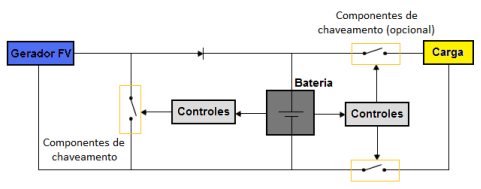
\includegraphics[width = .5 \textwidth]{energia/figuras/ene_pc1_14}
		\caption{Controlador de carga em paralelo. \cite{Cresesb}.}
		\label{ene_pc1_14}
	\end{figure}


	O componente utiliza um relé eletromecânico ou um dispositivo semicondutor para realizar o chaveamento. Quando a bateria atinge plena carga, a chave em paralelo se fecha criando um curto no painel, desta forma a maior parte da corrente produzida retorna ao gerador fotovoltaico e apenas uma fração segue em direção a bateria. \cite{Cresesb}.
	
	Assim como no caso anterior, nem todo modelo comercial apresenta as chaves entre a bateria e a carga para evitar descargas excessivas. Além disso, esse modelo necessita de um diodo de bloqueio para evitar perdas por corrente reversa durante a noite.
	
	Ambos os modelos anteriores utilizam a estratégia de controle “On/off” que consiste em desacoplar os painéis fotovoltaicos da bateria quando esta atinge carga plena.  

	\textbf{Controlador de carga PWM (Pulse Width Modulation)}

	O controlador de carga PWM é uma variação dos modelos anteriores (Geralmente do controlador em série), que utiliza uma arquitetura semelhante, porém aplica o método de controle de modulação por pulsos para aumentar a eficiência do sistema. \cite{Saad}.
	
	O controlador transmite a energia proveniente dos painéis para a bateria através de pulsos cíclicos que podem atingir frequências de centenas de ciclos por segundo. Desta forma, ela consegue manter a tensão das baterias em um nível mais constante e reduzir o tempo que os painéis permanecem desacoplados da bateria, consequentemente aumentando a eficiência do sistema. \cite{Saad}.

	\textbf{Controlador de carga MPPT (Maximum power point tracking)}

	Os controladores de carga MPPT são os mais eficientes, possuem arquitetura semelhante a apresentada anteriormente, porém contam com dispositivos sofisticados de eletrônica de potência para manter a transmissão de energia dos painéis para a bateria sempre no ponto máximo de eficiência. Isto é realizado, ajustando os valores de tensão e corrente provenientes do gerador fotovoltaico de modo a manter a potência transmitida. \cite{Cresesb}.
	
	Por exemplo, considere um painel fotovoltaico de 90 Wp com tensão nominal de 17,06 V e corrente nominal de 5,28 A (referência do painel sinosola SA90-64P). Caso seja utilizado um controlador de carga PWM de 12,5 V (Tensão de saída para bateria) a potência transmitida será de 12,5V * 5,28 totalizando 66 W, ou seja, apenas 73,3\% da potência será transmitida para a bateria. No caso do controlador MPPT há um aumento da corrente proporcional a diminuição da tensão necessária para alimentação da bateria, de modo que no caso anterior a corrente assumiria valores próximos a 9,14 A e a potência entregue a bateria se aproxime dos 90W.
	
	Segundo a CRESESB em seu Manual de Engenharia para Sistemas Fotovoltaicos de 2014, a eficiência do controle por MPPT está na faixa de 92 a 97\%. Porém, o custo deste tipo de controlador ainda é elevado.

\subsubsection{Definição da tecnologia que será usada no projeto}	

	Para o projeto será empregado um controlador de carga PWM. Embora apresente uma eficiência menor que o MPPT o que se reflete na necessidade de aumentar a potência gerada pelo gerador fotovoltaico, seu custo é cerca de cinco vezes menos do que o controlador por MPPT.
	
	Como o sistema fotovoltaico consiste de poucos painéis, a redução de custos no gerador fotovoltaico não compensa o aumento de custos no controlador. Além disso, a diferença de dimensões físicas e de peso entre o painel usado e o modelo diretamente inferior no quesito de geração não reduz consideravelmente os custos com a estrutura.

\subsubsection{Dimensionamento do controlador de carga} 

	Para o dimensionamento de um controlador de carga deve-se levar em conta a potência gerada pelos painéis fotovoltaicos e a tensão de operação do sistema de bateria. Assim, é possível calcular a corrente de trabalho do componente e escolher o modelo que melhor atenda a necessidade do projeto.
	
	Dessa forma, temos:

\begin{equation}
C_o = \dfrac{P_g}{V_{Banco}}
\end{equation}
	
	Sendo $C_o$ a corrente de operação, $P_g$ a potência gerada pelos painéis e $V_{Banco}$ a tensão do banco de baterias.
	
	Utilizando a corrente encontrada é possível definir o controlador necessário para a aplicação. Não é recomendado instalar sistemas que trabalhem em alta corrente, pois é necessário o aumento do diâmetro dos condutores, aumentasse as perdas por efeito joule e os controladores se tornam mais caros. Deste modo, dependendo da corrente de operação é recomendável separar o sistema em mais de um circuito utilizando mais de um controlador de carga.

\section{Sistema de acionamento das bombas} 

Um dos requisitos integrantes do projeto é realizar o acionamento do sistema de irrigação de forma automática caso o usuário decida por este modo. Assim, é necessário projetar um módulo de acionamento remoto que atue no quadro de comando do sistema de irrigação e esteja em paralelo com o sistema atual de acionamento.

Foi analisado a viabilidade de utilizar um módulo de acionamento industrial a distância utilizando frequência de rádio de modo a acionar a contatora e partir as bombas. Porém estes equipamentos possuem valores acima do orçamento de projeto, além de utilizarem módulos e protocolos prontos de comunicação dificultando a integração com o resto do sistema. Além do fato de que funcionam como uma caixa preta recebendo um input e tendo como saída um output fixo, de modo que não se entende bem como ocorre seu funcionamento interno.

Por causa disso optou-se por não utilizar esse tipo de sistema e invés disso construir um sistema próprio de acionamento a distância. As imagens a seguir apresentam o sistema proposto tanto do ponto de vista de um produto comercial quanto do que será implementado no projeto integrador 2.

	\begin{figure}[H]
		\centering
		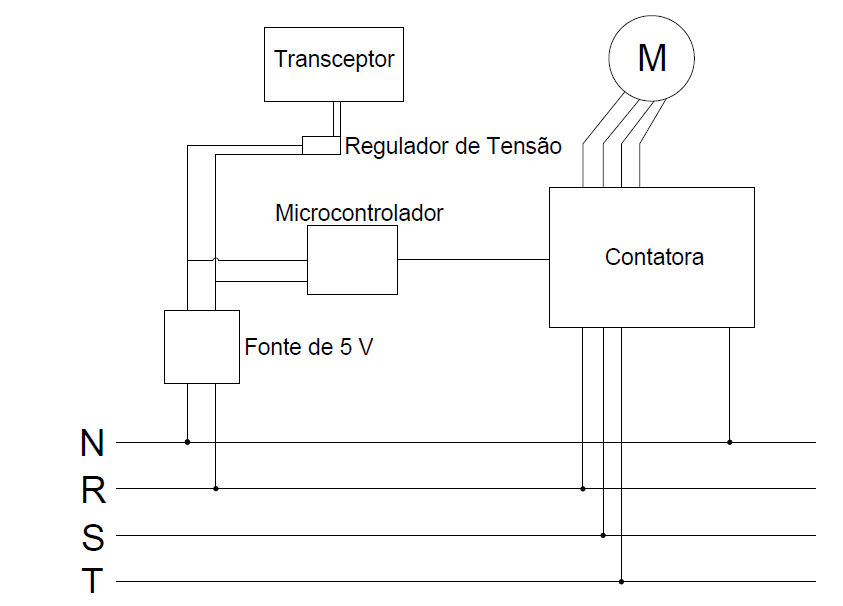
\includegraphics[width = .5 \textwidth]{energia/figuras/ene_pc1_15}
		\caption{Esquemático de acionamento da irrigação para o produto. Fonte: Do Autor}
		\label{ene_pc1_15}
	\end{figure}


	\begin{figure}[H]
		\centering
		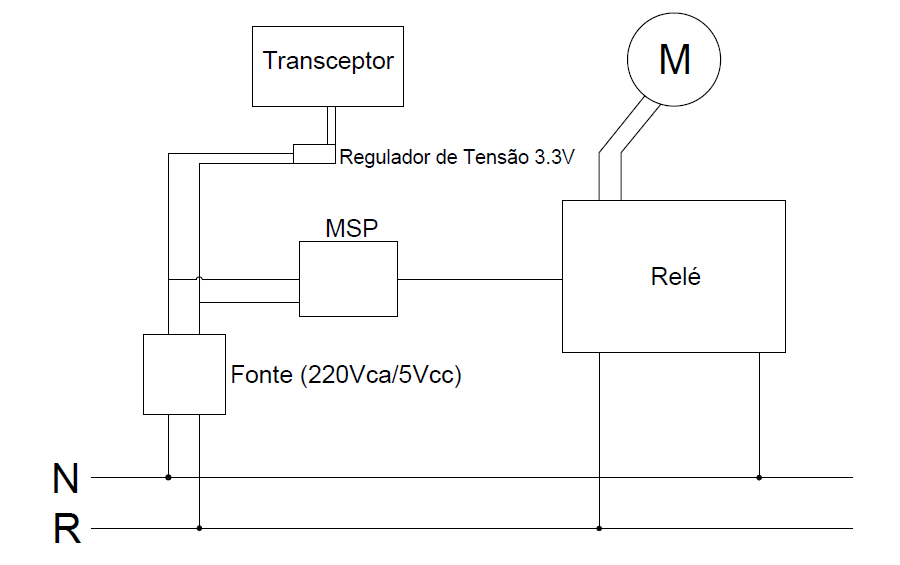
\includegraphics[width = .5 \textwidth]{energia/figuras/ene_pc1_16}
		\caption{Esquemático de acionamento da irrigação para o protótipo. Fonte: Do Autor}
		\label{ene_pc1_16}
	\end{figure}


Ambos os esquemáticos seguem a mesma ideia geral sendo que no projeto usaremos uma bomba monofásica para demonstrar o funcionamento do sistema e utilizaremos um relé no lugar da contatora de modo a reduzir os custos do protótipo.

No caso referente ao protótipo, será utilizado o mesmo transceptor utilizado no sistema de comunicação apresentado anteriormente. Além disso, será necessária uma fonte de alimentação para converter a tensão alternada de 220V para 5V em corrente contínua e um regulador de tensão que converta os 5V para 3.3V de modo a alimentar os componentes eletrônicos utilizados.

Para tal a fonte de alimentação utilizada será chaveada visando aumentar sua eficiência e será de 5V e lA. O regulador de tensão utilizado será o módulo Abaixador Tensão Ajustável DC-DC(LM2596).

O microcontrolador escolhido para processar o sinal recebido pelo transceptor será o MSP 430, pois o grupo já possui este equipamento e ele é capaz de executar o processamento do sinal e comandar o módulo relé. Tal módulo possuirá dois canais cada qual comandando um relé de 220V e 10A sendo um responsável por acionar ou desligar a bomba e o outro ficará desligado.

Por fim, será utilizada uma bomba de poço artesiano modelo 1650 da HS para simular o sistema de irrigação, tal bomba não faz parte do projeto em si, mas será usada para demonstrar o funcionamento do sistema de acionamento a distância.

\section{Dimensionamento preliminar sistema fotovoltaico}


Para determinação dos custos referentes ao sistema de alimentação foi necessário realizar um dimensionamento preliminar do sistema fotovoltaico da estação utilizando as equações apresentadas nesta seção. Tal dimensionamento foi uma estimativa realizada utilizando o consumo dos equipamentos eletrônicos como base e sofrerá alterações no decorrer do projeto visando sua adequação e melhoria.

A carga à ser alimentada foi estimada em 10 W e corresponde aos sensores e outros equipamentos da estação. De modo geral foi estimado que os sensores trabalham 24 horas por dia enquanto que os demais componentes como o cooler trabalham apenas 6 horas. Assim, foi possível calcular a energia a ser produzida diariamente pelos painéis fotovoltaicos através da equação:

\begin{equation}
E_p = \sum C.t.1,5
\end{equation}

Sendo C o consumo do componente, t o tempo de operação e "1,5" a taxa de dimensionamento utilizada para simular as perdas no controlador, regulador de tensão e outros pontos. 

Deste modo, obteve-se um necessidade de geração de 191,2 Wh por dia. Considerando a menor taxa de irradiação solar brasileira (4,44 kWh/$m^2$), denotada por I, foi possível calcular a potência do painel necessário através da equação:

\begin{equation}
P = \dfrac{E_p}{I}
\end{equation}

Assim, obteve-se que o painel solar deveria gerar 43 Wp. O modelo comercial que foi escolhido foi de 60 W, pois ela supre a produção calculada e possui valor inferior aos modelos de 50 e 55 W encontrados.

Para dimensionamento da bateria utilizou-se a seguinte equação:

\begin{equation}
CB_{c20} = \dfrac{E_p . N}{V_{bat}}
\end{equation} 

A autonomia do sistema foi definida como três dias e não se levou em conta a taxa de descarga, pois como o projeto trata se de um protótipo do sistema não é necessário que a vida útil da bateria seja tão longa quanto em um caso real. Caso a profundidade de descarga fosse considerada a bateria se tornaria muito cara ultrapassando o orçamento definido. 

Assim obteve-se que uma bateria de 26 Ah supriria o sistema.

Para a definição dos disjuntores e do controlador de carga utilizou-se as informações de corrente de curto circuito do painel de modo que foi escolhido utilizar um controlador de carga de 5A e disjuntores de 5A para proteger o sistema e interromper a energia durante as manutenções. 

Os demais componentes levantados para construção do sistema de alimentação estão disponíveis no anexo de custos do sistema.

Todo o procedimento de cálculo e escolha dos componentes será melhor detalhado no próximo ponto de controle de modo a ser refinado e atualizado com as novas informações do projeto.













